\chapter{Progettazione e architettura}
\label{chap:progettazione-architettura}

\section{Architettura generale}
\label{sec:architettura-generale}
\noindent La progettazione dell'architettura del sistema è stata guidata da diversi principi chiave, tra cui modularità, scalabilità e manutenibilità. Per garantire la corretta interazione tra l'applicazione mobile e i sistemi aziendali preesistenti, il sistema è stato suddiviso in macro-componenti distinti, ognuno con responsabilità ben definite. Come illustrato nello schema generale \ref{fig:architettura}, il sistema si compone di quattro blocchi principali:
\begin{itemize}
    \item \textbf{App Mobile (Frontend)}: sviluppata in \gls{dotnetmauig}, rappresenta l'interfaccia con cui il dipendente interagisce. Si occupa di raccogliere gli input dell'utente, gestire la fotocamera per l'acquisizione delle foto e applicare le prime logiche di validazione dei dati.
    \item \textbf{Database Locale}: integrato direttamente all'interno del dispositivo mobile tramite \gls{sqliteg}, funge da archivio temporaneo per i dati raccolti dall'app. Permette all'applicazione di funzionare anche in assenza di connettività, garantendo la memorizzazione sicura e organizzata delle informazioni prima della sincronizzazione con il \textit{backend}.
    \item \textbf{Web Services ed ERP Ergon (Backend)}: rappresentano l'infrastruttura di \textit{backend} centrale dell'azienda. Il livello \textit{Services} dell'applicazione mobile comunica con questa componente per inviare i dati elaborati delle note spesa e ricevere le conferme di storicizzazione nel database centrale. 
    \item \textbf{Servizio Cloud AI}: \gls{azurecontentunderstandingg} è la componente esterna interrogata dal \textit{backend} dell'applicazione. Quest'ultima si limita a inoltrare l'immagine per poi ricevere in risposta i dati estratti in formato strutturato, delegando completamente l'onere computazionale all'esterno del dispositivo.
\end{itemize}

\begin{figure}[H]
    \centering
    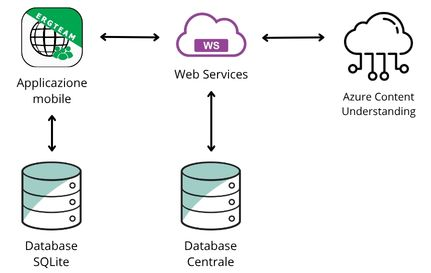
\includegraphics[width=0.7\textwidth]{img/architetturasistema.jpg}
    \caption{Architettura ad alto livello del sistema.}
    \label{fig:architettura}
\end{figure}

\noindent Il flusso tipico dei dati prevede che l'informazione nasca sul dispositivo mobile, venga salvata nel database locale e, non appena vi è disponibilità di rete, venga inviata ai web services per la storicizzazione finale.


\section{Struttura del progetto}
\noindent Per mantenere il codice ordinato e favorirne la manutenibilità da parte del team di sviluppo di Ergon, la struttura del progetto è stata organizzata seguendo le convenzioni aziendali e rispecchiando i principi del pattern architetturale scelto. \\
All'interno della cartella principale dell'applicazione, il codice è stato suddiviso nelle seguenti cartelle logiche:
\begin{itemize}
    \item \textbf{Models}: contiene le classi \gls{csharpg} che rappresentano le entità del dominio applicativo, la struttura dei dati e mappano fedelmente la struttura delle tabelle del database locale.
    \item \textbf{Views}: ospita tutti i file scritti in linguaggio \gls{xamlg} che definiscono l'interfaccia utente e gli elementi visivi dell'applicazione. Ogni file \gls{xamlg} è accompagnato dal rispettivo file di \textit{code-behind} in \gls{csharpg}, che gestisce la logica di interazione e gli eventi associati agli elementi dell'interfaccia. 
    \item \textbf{ViewModels}: rappresentano il cuore logico dell'interfaccia. Contiene le classi \gls{csharpg} che preparano i dati per le \textit{Views} e gestiscono le azioni dell'utente tramite comandi e proprietà \textit{bindate}. Questa cartella incarna il pattern \gls{mvvm}, separando nettamente la logica di presentazione dalla logica di business.
    \item \textbf{Services}: raggruppa i componenti responsabili della comunicazione con i servizi esterni e della gestione dei dati, operando come strato intermedio tra il \textit{frontend} e il \textit{backend}. Al suo interno sono presenti: 
    \begin{itemize}
        \item \textit{RestService}: gestisce la comunicazione con il server aziendale, occupandosi dell'autenticazione dell'utente, della sincronizzazione dei dati, dell'invio delle note spesa e dell'inoltro degli allegati destinati al servizio di analisi automatica.
        \item \textit{ErgDatabase}: fornisce l'accesso al database locale e centralizza le operazioni di persistenza dei dati. Garantisce la corretta gestione delle transazioni e degli accessi concorrenti alle risorse condivise, assicurando l'integrità delle informazioni memorizzate.
        \item \textit{MediaService}: si occupa dell'elaborazione degli allegati multimediali acquisiti dall'utente, eseguendo operazioni di normalizzazione, ottimizzazione e compressione delle immagini al fine di ridurre il consumo di banda e rispettare i vincoli dimensionali previsti dall'infrastruttura aziendale.
        \item \textit{Settings}: gestisce la persistenza delle preferenze dell'utente e dello stato globale dell'applicazione, fornendo un'interfaccia unificata per l'accesso alle impostazioni memorizzate sul dispositivo.
    \end{itemize}
\end{itemize}
Questa suddivisione garantisce un elevato grado di coesione interna e un basso accoppiamento tra le parti, permettendo di isolare le responsabilità e facilitare la manutenzione futura del codice da parte del team di sviluppo.


\section{Il pattern MVVM in pratica}
\noindent Per garantire un'architettura frontend solida, manutenibile e facilmente testabile, l'applicazione mobile è stata ingegnerizzata seguendo il pattern architetturale \gls{mvvm}, lo standard di riferimento per le applicazioni sviluppate con il framework \gls{dotnetmauig}.
Come anticipato durante l'analisi della struttura del progetto, l'obiettivo principale di questa scelta è la separazione delle responsabilità. Avendo già suddiviso il codice in modelli logici, viste grafiche e classi di orchestrazione intermedie, il pattern definisce regole rigide con cui questi tre livelli devono interagire senza accoppiarsi, come schematizzato in figura \ref{fig:mvvm}.

\begin{figure}[H]
    \centering
    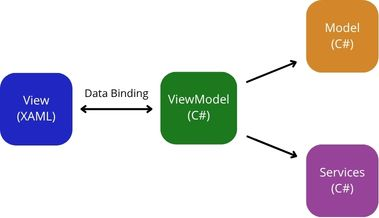
\includegraphics[width=0.65\textwidth]{img/mvvm.jpg}
    \caption{MVVM pattern applicato al progetto.}
    \label{fig:mvvm}
\end{figure}

\subsection*{Data Binding e comandi}
\noindent Uno degli elementi centrali del pattern è il meccanismo di comunicazione bidirezionale tra la \textit{View} e il \textit{ViewModel}, noto come \textit{Data Binding}. \\
Invece di scrivere codice per aggiornare manualmente un'etichetta di testo o per leggere il valore di un input, l'interfaccia grafica viene "legata" in modo dichiarativo alle proprietà del \textit{ViewModel}. Quando, ad esempio, il motore di sincronizzazione in background aggiorna lo stato di una nota spesa nel \textit{ViewModel}, la \textit{View} si aggiorna in tempo reale e in totale autonomia, reagendo al cambiamento di stato senza che la logica di business debba manipolare direttamente gli elementi visivi. \\
Allo stesso modo, le azioni dell'utente (come il tap su un pulsante per il salvataggio o per l'apertura della fotocamera) non innescano direttamente funzioni nel \textit{code-behind} della \textit{View}, ma sono mappate tramite il meccanismo dei \textit{Command}. Un \textit{Command} è un'istruzione esposta dal \textit{ViewModel} che la \textit{View} si limita a richiamare. Questo approccio ha permesso di centralizzare tutta la logica di reazione agli input dell'utente all'interno del \textit{ViewModel}, rendendo il comportamento dell'applicazione estremamente coerente. \\
Questa netta separazione garantisce vantaggi significativi per il ciclo di vita del software: facilita il lavoro in team, rende il codice altamente riutilizzabile e getta le basi per l'implementazione di test automatici sulla logica dell'interfaccia senza dover simulare la reale interazione dell'utente con lo schermo del dispositivo.


\section{Progettazione dell'interfaccia}
\noindent La progettazione dell'esperienza utente (\textit{UX}) è stata un aspetto cruciale del processo di sviluppo, poiché l'applicazione è destinata a essere utilizzata quotidianamente da un ampio numero di dipendenti con diversi livelli di familiarità tecnologica. L'obiettivo principale è stato quello di creare un'interfaccia intuitiva, semplice da navigare e che minimizzasse il numero di passaggi necessari per completare le operazioni più comuni, come la creazione e l'invio di una nota spesa. \\
Una strategia adottata è stata quella di privilegiare l'uso di dialoghi modali e finestre di conferma per le operazioni secondarie o di supporto, invece che forzare l'utente a cambiare continuamente schermata. Questa scelta riduce il carico cognitivo dell'utente e mantiene il focus sull'attività principale, migliorando l'efficienza e la soddisfazione complessiva nell'utilizzo dell'applicazione.


\section{Progettazione dei modelli di dati}
\noindent La persistenza, lo scambio e la consistenza delle informazioni all'interno del sistema richiedono una progettazione accurata delle entità di dominio. Nel contesto di un'architettura \textit{client-server} progettata per funzionare anche in assenza di rete, la modellazione dei dati è stata effettuata rispondendo a due esigenze principali: garantire la leggerezza delle operazioni sul dispositivo mobile e assicurare la conformità con le regole dei database aziendali centrali. \\
Per raggiungere questi obiettivi, sono state definite diverse classi \gls{csharpg} che rappresentano le entità chiave del dominio applicativo, andando a implementare differenze specifiche tra lo strato di \textit{frontend} e quello di \textit{backend} per adattarsi ai rispettivi contesti operativi. 

\subsection*{La modellazione della Nota spesa}
\noindent Il fulcro informativo dell'applicazione è rappresentato dalla singola riga di spesa. Questa entità descrive ogni transazione eseguita dal dipendente e contiene tutte le informazioni necessarie per la corretta gestione del processo di rendicontazione. Nel \textit{frontend} mobile, il modello dati è stato esteso per supportare la logica offline. Oltre ai campi essenziali di business, l'entità include:
\begin{itemize}
    \item \textbf{Doppia indicizzazione}: ogni nota spesa possiede un identificativo locale, necessario per salvare e gestire il record sul dispositivo anche senza rete, e un identificativo remoto, inizialmente uguale a zero e aggiornato solo dopo conferma di ricezione e storicizzazione del dato da parte del \textit{backend}.
    \item \textbf{Flag di stato}: proprietà booleana utilizzata dall'applicazione per distinguere istantaneamente le note spesa già sincronizzate da quelle che richiedono un invio al server.
    \item \textbf{Gestione ibrida dei file}: il modello tiene traccia sia del percorso fisico della foto dello scontrino salvata temporaneamente sulla memoria del dispositivo, sia dell'\gls{urlg} relativo che il file assumerà una volta caricato sul server aziendale.
\end{itemize}
\noindent Specularmente, sul \textit{backend} aziendale, l'entità corrispondente è modellata senza tutte queste logiche di supporto. Il server riceve i dati, li valida e li mappa direttamente sulla struttura del database centrale, utilizzando esclusivamente i propri identificativi e le proprie convenzioni di storicizzazione.

\subsection*{Dizionari dati e vincoli di standardizzazione}
\noindent Per garantire la qualità del dato inserito dall'utente e prevenire errori di compilazione, l'architettura fa uso di tabelle di decodifica. Invece di permettere l'inserimento libero di testo per campi come la tipologia di spesa o il metodo di pagamento, l'applicazione mobile scarica all'avvio i dizionari validi direttamente dall'\gls{erp} aziendale. Questi modelli ausiliari assicurano che una nota spesa creata sul dispositivo rispetti sempre i vincoli amministrativi ancor prima di essere inviata, delegando al client una prima fase di validazione.

\subsection*{DTO per l'Intelligenza Artificiale}
\noindent Un'ulteriore accortezza progettuale ha riguardato la gestione dei dati di ritorno dal servizio \textit{Cloud AI}. Per questa interazione è stato progettato un modello specifico, che agisce come un puro \gls{dtog}. Questo oggetto è privo di chiavi primarie o logiche di persistenza locale: serve unicamente come contenitore volatile per far transitare in modo strutturato i dati ricevuti in risposta dall'\gls{ia} dall'infrastruttura di rete fino alla \textit{View}, permettendo all'utente di visualizzarli prima dell'effettivo salvataggio nel database.


\section{Progettazione del database locale}
\noindent Come definito nelle scelte tecnologiche nella sezione \ref{sec:persistenza-sincronizzazione}, la persistenza dei dati sul dispositivo mobile è delegata a \gls{sqliteg}.
Per garantire un funzionamento fluido e reattivo dell'applicazione, lo schema del database è stato progettato mantenendo un adeguato livello di normalizzazione, ma limitando il numero di entità allo stretto necessario per il dominio mobile. L'obiettivo principale è fornire un supporto alla creazione, modifica e storicizzazione temporanea delle note spesa in modalità offline. Per questo motivo, la base dati replica localmente solo i vincoli di integrità e i dizionari indispensabili per la validazione dell'input utente, senza appesantire il dispositivo con l'intera complessità relazionale dell'\gls{erp} centrale.

\begin{figure}[H]
    \centering
    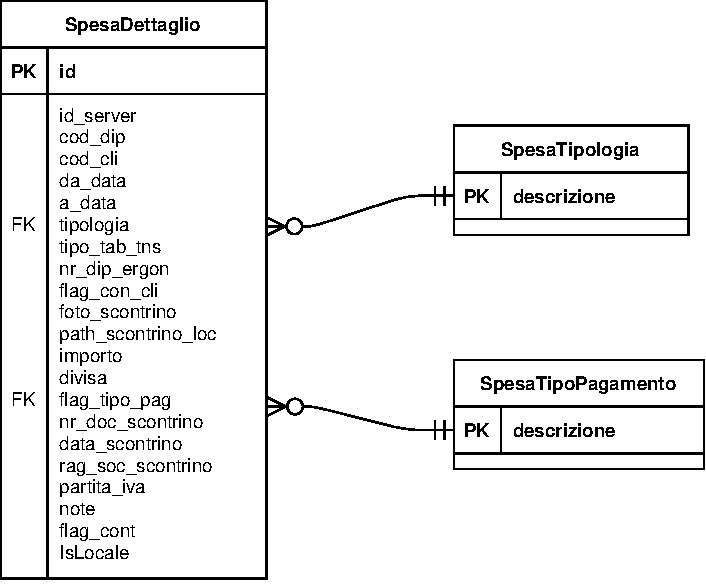
\includegraphics[width=0.7\textwidth]{img/database.pdf}
    \caption{Schema del database locale.}
    \label{fig:db_locale}
\end{figure}

\subsection*{Struttura relazionale}
\noindent Come illustrato nello schema in figura \ref{fig:db_locale}, il database locale è stato strutturato in modo essenziale, suddividendo le tabelle in due macro-categorie funzionali. Da un lato vi sono le tabelle di decodifica, \textit{SpesaTipologia} e \textit{SpesaTipoPagamento}, che sono in sola lettura per l'utente e fungono da dizionari per i vincoli di integrità. Dall'altro vi è la tabella operativa principale, \textit{SpesaDettaglio}, che costituisce il nucleo transazionale dell'app in cui vengono registrate le note spese. I campi \textit{tipologia} e \textit{flag\_tipo\_pag} agiscono come chiavi esterne per vincolare l'inserimento ai soli valori autorizzati dall'\gls{erp} aziendale. Inoltre, il database viene generato in modo dinamico: al primo avvio dell'applicazione, il servizio verifica l'esistenza dell'archivio sul dispositivo e, in caso negativo, costruisce automaticamente lo schema delle tabelle basandosi sui modelli \gls{csharpg}.

\subsection*{Approccio a oggetti}
\noindent L'interazione tra l'applicazione e il database non avviene tramite query testuali dirette, ma è mediata da un framework \gls{ormg}. Questa scelta progettuale ha permesso di mappare automaticamente i modelli dati descritti in precedenza (le classi \gls{csharpg}) nelle rispettive tabelle relazionali. L'utilizzo di un \gls{orm} eleva il livello di astrazione: il team di sviluppo può manipolare i record del database come se fossero normali oggetti in memoria, delegando al framework la traduzione di queste operazioni nel linguaggio \textit{SQL} sottostante. Ciò riduce drasticamente la probabilità di errori sintattici e facilita la manutenzione futura.

\subsection*{Gestione della concorrenza e reattività dell'interfaccia}
\noindent In un'applicazione mobile moderna, l'esperienza utente non deve essere interrotta da blocchi dell'interfaccia grafica o da operazioni di accesso alle risorse del dispositivo. Per questo motivo, l'intera architettura del database locale è stata progettata per essere asincrona, che consente di eseguire le operazioni di lettura e scrittura senza bloccare il thread principale dell'interfaccia. 
Ogni interrogazione o salvataggio viene quindi eseguito in background, mantenendo l'applicazione reattiva anche durante attività intensive come la sincronizzazione dei dati o il salvataggio di allegati multimediali. \\
Per garantire la consistenza delle informazioni memorizzate, l'accesso al database è centralizzato attraverso un'unica istanza condivisa della connessione. Inoltre, specifici meccanismi di sincronizzazione impediscono accessi concorrenti non controllati alle risorse, evitando possibili conflitti tra operazioni simultanee.


\section{Sicurezza e comunicazione}
\noindent Trattandosi di un'applicazione aziendale che gestisce dati sensibili e informazioni contabili, la sicurezza della comunicazione tra il dispositivo mobile e i server centrali ha rappresentato un requisito architetturale imprescindibile.
L'intero scambio di informazioni è protetto tramite protocolli crittografati (\textit{HTTPS}), che garantiscono l'integrità e la riservatezza dei dati in transito, comprese le immagini degli scontrini acquisite dalla fotocamera. Inoltre, l'accesso ai servizi web esposti dall'\gls{erp} aziendale è vincolato da meccanismi di autenticazione restrittivi. Il livello dei servizi dell'applicazione si occupa di gestire la validazione e l'inserimento automatico delle credenziali in ogni singola richiesta di rete, assicurando che esclusivamente i dipendenti autorizzati e regolarmente censiti a sistema possano inviare, scaricare e sincronizzare i propri report di spesa.


\newpage